%
% $Id: $
%

%\documentclass[times,10pt,twocolumn]{article}
%\documentclass[times,12pt]{article}
\documentclass[a4paper,11pt]{article}
\usepackage[utf8]{inputenc}
\usepackage{times}

%\documentstyle[times,art12,format/latex8]{article}

\usepackage{url}
\usepackage{subfigure}
\usepackage{amssymb}
\usepackage{amsmath}
\usepackage{psfrag}
\usepackage{epsfig}
\usepackage{graphicx}
\usepackage{graphics}

% COMMENTS (optional argument is author of comment)
\newcommand{\comments}[2][?]{
  \begin{quote}
    \textbf{Comment (#1):} {\em #2}
  \end{quote}
  }
%% Uncomment this line to remove comments
%\renewcommand{\comments}[2][?]{}


%-------------------------------------------------------------------------
% take the % away on next line to produce the final camera-ready version
\pagestyle{empty}

%-------------------------------------------------------------------------
\begin{document}

\title{Protocolos para la Transmisión de Audio y Vídeo por Internet\\ 
\ \\ 
Práctica Final \\
(Versión v5.0, 30.11.2014) % \\
%\ \\
%\footnotesize{Nota: Es probable que el guión de la práctica final varíe en las
%próximas semanas, principalmente durante los primeros días, añadiendo puntualizaciones y aclaraciones.}
}

\maketitle
\thispagestyle{empty}
\tableofcontents
\newpage

%-------------------------------------------------------------------------

\section{Introducción}

Esta práctica tiene como objetivo implementar los programas en Python 
necesarios para realizar una sesión SIP de intercambio de audio vía RTP
como la que se muestra en la siguiente figura\footnote{Los métodos SIP
aparecen en mayúsculas en la figura, por claridad. En la práctica, siguiendo
el RFC, sólo la primera letra de cada palabra ha de ser mayúscula.}:

\begin{center}
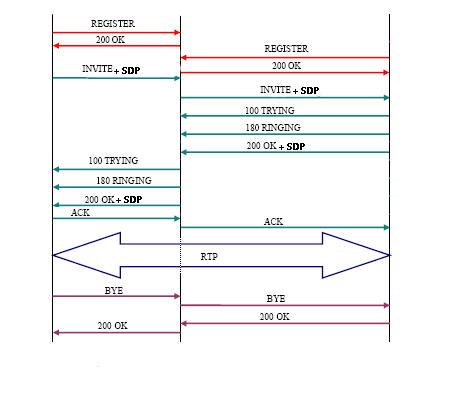
\includegraphics{figs/complete-sip-session.png}
\end{center}

En esta sesión:

\begin{itemize}
  \item El UA de la izquierda constará de una parte cliente y otra servidora (se puede partir de los programas realizados en la práctica 6).
  \item El UA de la derecha constará de una parte cliente y otra servidora (se puede partir de los programas realizados en la práctica 6).
  \item Habrá un servidor de registro (se puede partir del programa realizado en la práctica 4) y de \emph{proxy}, que intermediará únicamente en el intercambio SIP; los paquetes RTP irán directamente de UA emisor a UA receptor, sin pasar por el proxy/registrar.
\end{itemize}


\subsection{Conocimientos previos necesarios}

\begin{itemize}
  \item Nociones de SIP (las de clase de teoría)
  \item Funcionamiento de wireshark
\end{itemize}

Tiempo estimado: 25 horas


\subsection{Entrega}

Con el navegador, dirígete al repositorio \texttt{ptavi-pfinal} en la cuenta del profesor en GitHub\footnote{\url{http://github.com/gregoriorobles/ptavi-pfinal}} y realiza un \texttt{fork}, de manera que consigas tener una copia del repositorio en tu cuenta de GitHub. Clona el repositorio que acabas de crear a local para poder editar los archivos. Trabaja a partir de ahora en ese repositorio, sincronizando los cambios que vayas realizando.

Se proporciona un script de comprobación de entrega correcta, \emph{check-pfinal.py}. Es responsabilidad del alumno comprobar la correcta entrega mediante este script.

La entrega de práctica se deberá hacer antes del {\bf día límite de entrega a las 23:55}\footnote{El día límite en esta versión del documento todavía no se conoce.}. Para entonces, se debe tener un repositorio git en GitHub con los siguientes archivos:

\begin{enumerate}
  \item uaclient.py
  \item uaserver.py
  \item proxy\_registrar.py
  \item ua1.xml (con un ejemplo de fichero de configuración del UA)
  \item ua2.xml (con otro ejemplo de fichero de configuración del UA)
  \item pr.xml (con un ejemplo de fichero de configuración del proxy/registrar)
  \item llamada.libpcap
  \item error.libpcap
  \item avanzadas.txt (fichero opcional, sólo necesario en caso de realizar algún requisito avanzado)
  \item passwords.txt (fichero opcional, sólo necesario en caso de realizar el requisito avanzado de registro seguro)
\end{enumerate}

Otras consideraciones:
\begin{itemize}
  \item Se tendrá en cuenta para la nota de la práctica la adecuación de los
programas Python a la guía de estilo de Python PEP-8.
  \item Se valorará el uso de git (frecuencia de commits y adecuación de los comentarios de cada commit).
  \item Se valorará que la práctica siga las
convenciones indicadas en este documento, en particular que el intercambio
de mensajes, los parámetros de los programas y los mensajes en el fichero de \emph{log} sean los
que especifican. En la \texttt{shell} pueden incluirse las trazas que el alumno desee y en el formato que le parezca más conveniente.
  \item Se valorará que las capturas estén bien filtradas y sólo contengan los paquetes que se indican en el guión.
  \item Se valorará que el equipo al que pertenece el alumno siga la guía de estilo
de Python, tenga código legible y bien estructurado.
  \item Se valorará que el cliente y el servidor funcione con los miembros del equipo. Sólo en los casos en los que se realizan requisitos avanzados incompatibles, esta consideración no se tendrá en cuenta.
  \item Se pasará un programa anti-copia a las prácticas entregadas.
\end{itemize}


\section{User Agent}

Cada \emph{User Agent} deberá constar de una parte cliente y otra servidora, que podrán estar ubicados en programas Python diferentes (y, por tanto, requerirán de dos terminales para ser ejecutados).

\subsection{Configuración}

La configuración del \emph{User Agent} estará almacenada en un fichero
con formato XML válido, que seguirá 
la sintaxis que se describe en el  siguiente DTD\footnote{Se puede profundizar en la sintaxis de las DTD en: http://www.javadabbadoo.org/apendice/dtd/sintaxis/index.html}:

\begin{verbatim}
<!ELEMENT config (account, uaserver, rtpaudio, regproxy, log, audio)>
<!ELEMENT account EMPTY>
<!ATTLIST account username CDATA #REQUIRED>
<!ATTLIST account passwd CDATA #IMPLIED>
<!ELEMENT uaserver EMPTY>
<!ATTLIST uaserver ip CDATA #IMPLIED>
<!ATTLIST uaserver puerto CDATA #REQUIRED>
<!ELEMENT rtpaudio EMPTY>
<!ATTLIST rtpaudio puerto CDATA #REQUIRED>
<!ELEMENT regproxy EMPTY>
<!ATTLIST regproxy ip CDATA #REQUIRED>
<!ATTLIST regproxy puerto CDATA #REQUIRED>
<!ELEMENT log EMPTY>
<!ATTLIST log path CDATA #REQUIRED>
<!ELEMENT audio EMPTY>
<!ATTLIST audio path CDATA #REQUIRED>
\end{verbatim}

donde los elementos son los siguientes:

\begin{itemize}
  \item account: Cuenta del usuario, con su nombre y opcionalmente su contraseña.
  \item uaserver: Lugar de escucha de la parte servidora del \emph{User Agent}, indicando su dirección IP (opcional, en caso de no estar indicada se utilizará 127.0.0.1) y el puerto.
  \item rtpaudio: Puerto de recepción para el audio RTP.
  \item regproxy: Parámetros de localización del servidor Proxy/Registrar: IP y puerto.
  \item log: Localización (\emph{path}) del fichero de log del \emph{User Agent}.
  \item audio: Localización (\emph{path}) del fichero MP3.
\end{itemize}

\subsection{Log}


El cliente ha de escribir mensajes de depuración y de \emph{log} en un fichero indicado en el fichero XML de configuración. Cada línea de este fichero de log ha de tener un mensaje con el que se pueda trazar qué es lo que ha ocurrido (o está ocurriendo) en el \emph{User Agent}.

Los ficheros de log deben tener la siguiente estructura:


\begin{footnotesize}
\begin{verbatim}
Tiempo en formato YYYYMMDDHHMMSS (espacio en blanco) Evento
\end{verbatim}
\end{footnotesize}

donde evento puede ser:

\begin{itemize}
  \item En caso de envío: \emph{Sent to \texttt{IP:port}: mensaje completo en una única línea}. Los saltos de línea han de transformarse en espacios en blanco.
  \item En caso de recepción: \emph {Received from \texttt{IP:port}: mensaje completo en una única línea}. Los saltos de línea han de transformarse en espacios en blanco.
  \item En caso de error (p.ej. porque se ha enviado algo a un puerto que no está escuchando): \emph{Error: mensaje de error en una única línea}. Los saltos de línea han de transformarse en espacios en blanco.
  \item Otros eventos: Tipo de evento, tal como \emph{Starting...}, \emph{Finishing.}, etc.
\end{itemize}


Nótese que cada línea ha de contener la fecha en el formato indicado, luego
un espacio en blanco y luego una de las siguientes. Un ejemplo de un fichero que siga esta estrucura es:

\begin{footnotesize}
\begin{verbatim}
...
20101018152045 Starting...
20101018153012 Sent to 127.0.0.1:5555: REGISTER sip:leonard@bigbang.org:1234 SIP/2.0 [...]
20101018153017 Received from 127.0.0.1:5555: 200 OK [...]
20101018153036 Sent to 127.0.0.1:5555: INVITE penny@girlnextdoor.com [...]
...
20101018160035 Sent to 127.0.0.1:5555: BYE [...]
20101018160035 Received from 127.0.0.1:5555: 200 OK [...]
20101018160112 Finishing.
\end{verbatim}
\end{footnotesize}

%\begin{itemize}
%  \item \emph{Starting...}: en caso de lanzar el programa.
%  \item \emph{Sent to IP:puerto: mensaje}: el mensaje enviado a la IP y puerto indicados, y a continuación el mensaje en sí. Todo en la misma línea (para ello, los saltos de línea se han de transformar en espacios en blanco).
%  \item \emph{Received from IP:puerto: mensaje}: el mensaje recibio desde la IP y puerto indicados, y a continuación el mensaje en sí. Todo en la misma línea (para ello, los saltos de línea se han de transformar en espacios en blanco).
%  \item \emph{Error: mensaje}: un mensaje de error (p.ej. porque se ha enviado algo a un puerto que no está escuchando.
%  \item \emph{Finishing}: en caso de terminar el programa.
%\end{itemize}

\subsection{User Agent Client (UAC)}

El cliente ha de ejecutarse de la siguiente manera:
\begin{verbatim}
  $ python uaclient.py config metodo opcion
\end{verbatim}

donde \emph{config} será un fichero XML con la configuración,
emph{metodo} será un método SIP, y \emph{opcion} será un parámetro
opcional dependiendo del método utilizado.

Por ejemplo:
\begin{verbatim}
  $ python uaclient.py ua1.xml REGISTER 3600
  $ python uaclient.py ua1.xml INVITE penny@girlnextdoor.com
  $ python uaclient.py ua1.xml BYE penny@girlnextdoor.com
  $ python uaclient.py ua1.xml REGISTER 0
\end{verbatim}

En caso de no introducir el número de parámetros correctos o de error en los mismos, el programa debería imprimir:
\begin{verbatim}
Usage: python uaclient.py config method option
\end{verbatim}

En caso de que se intentara establecer una conexión con un puerto no abierto
(p.ej. porque el servidor no haya sido lanzado), se capturará la excepción y, antes de finalizar el programa, se incluirá en el log un texto como el siguiente:
\begin{verbatim}
20101018160243 Error: No server listening at 193.147.73 port 5555
\end{verbatim}

El cliente podrá imprimirá por pantalla trazas, si así se desea. Se recuerda que 
los mensajes que envíe y reciba de sus comunicaciones han de aparecer
en el archivo de \emph{log} con el formato especificado con anterioridad.

\subsubsection{Métodos}

  \begin{itemize}
    \item REGISTER sip:emisor:puerto SIP/2.0

    Con este método el \emph{User Agent} se registra en un servidor de registro. Debido a las circunstancias donde se van a realizar las prácticas -donde los \emph{User Agents} van a estar ejecutándose en la misma máquina- debemos especificar el puerto de escucha del \emph{User Agent} en la petición.

    En las cabeceras del REGISTER ha de incluirse siempre una cabecera con el tiempo de expiración.

\begin{verbatim}
REGISTER sip:leonard@bigbang.org:1234 SIP/2.0
Expires: 3600
\end{verbatim}


    \item INVITE sip:receptor SIP/2.0

    Mediante este método, se indica que queremos iniciar una conversación con el receptor con dirección receptor en la máquina dada por la IP (que puede ser 127.0.0.1).

    El cuerpo del INVITE debe incluir la descripción de sesión en formato
 SDP (\emph{Session Description Protocol}), por lo que habrá que añadir la cabecera correspondiente al INVITE (Content-Type: application/sdp). Contará con los siguientes parámetros:

\begin{itemize}
  \item v (versión, por defecto la ``0''),
  \item o (originador e identificador de sesión: la dirección del originador y su IP),
  \item s (nombre de la sesión, que puede ser el que se desee),
  \item t (tiempo que la sesión lleva activa, en nuestro caso, siempre 0), y
  \item m (tipo de elemento multimedia y puerto de escucha y protocolo de transporte utilizados, en esta práctica ``audio'', el número de puerto pasado al programa principal como parámetro y ``RTP'').
\end{itemize}

Así, un ejemplo de descripción de sesión dentro de un INVITE podría ser:

\begin{verbatim}
INVITE sip:penny@girlnextdoor.com SIP/2.0
Content-Type: application/sdp

v=0
o=leonard@bigbang.org 127.0.0.1
s=misesion
t=0
m=audio 34543 RTP
\end{verbatim}

Nótese que en el ejmplo anterior 34543 es el puerto donde esperamos que el otro participante en la conversación nos envíe los paquetes RTP con audio. También se ha de tener en cuenta que entre las cabeceras (en este caso la línea de INVITE) y el cuerpo (la descripción de la sesión) ha de haber obligatoriamente una línea en blanco.

    \item ACK sip:receptor SIP/2.0

    Método de asentimiento. No se pasará al programa uaclient.py como parámetro, ya que se enviará una vez se hayan recibido las respuestas \emph{100 Trying}, \emph{180 Ringing} y \emph{200 OK} de la parte servidora tras hacerle un INVITE.

    \item BYE sip:receptor SIP/2.0

    Mediante este método se indica que queremos terminar la conversación que estamos manteniendo con la otra parte. Se deberá llamar, una vez haya acabado el streaming de audio vía RTP. Puede ser llamada desde cualquiera de los dos \emph{User Agents} involucrados en la conversación.

  \end{itemize}


\subsection{User Agent Server (UAS)}

El servidor ha de ejecutarse de la siguiente manera:
\begin{verbatim}
  $ python uaserver.py config
\end{verbatim}

donde \emph{config} será un fichero XML con los parámetros de configuración.

Por ejemplo:
\begin{verbatim}
  $ python uaserver.py ua1.xml
\end{verbatim}

En caso de no ejecutarse correctamente, el programa debería imprimir:
\begin{verbatim}
Usage: python uaserver.py config
\end{verbatim}

En caso contrario, el servidor imprimirá por pantalla:
\begin{verbatim}
Listening...
\end{verbatim}

El servidor podrá imprimir trazas por pantalla. Se recuerda que 
los mensajes que envíe y reciba de sus comunicaciones han de aparecer
en el archivo de \emph{log} en el formato especificado con anterioridad.

\subsubsection{Códigos de respuesta}

Los códigos de respuesta que el UA maneja han de ser, al menos, los siguientes:

   \begin{itemize}
     \item SIP/2.0 100 Trying: al recibir un INVITE.
     \item SIP/2.0 180 Ringing: al recibir un INVITE.
     \item SIP/2.0 200 OK: Deberá incluir SDP en el cuerpo (con su correspondiente cabecera de Content-Type).
     \item SIP/2.0 400 Bad Request: si la petición está mal formada.
     \item SIP/2.0 405 Method Not Allowed: si se manda en la petición cualquier otro método diferente de INVITE, BYE o ACK.
   \end{itemize}

\subsubsection{Envío RTP}

El envío RTP se realizará mediante el programa \texttt{mp32rtp} (como en la práctica 6). 
Para ejecutar instrucciones de \texttt{shell} desde Python, se puede utilizar algunos métodos del módulo os, en particular con \texttt{system()}. El parámetro que se le pasa a system es
el mandato de \texttt{shell} que se ha de ejecutar.

\begin{verbatim}
import os

# aEjecutar es un string con lo que se ha de ejecutar en la shell
aEjecutar = "./mp32rtp -i " + receptor_IP + " -p " + receptor_Puerto 
aEjecutar += " < " + fichero_audio

print "Vamos a ejecutar", aEjecutar
os.system(aEjecutar)
\end{verbatim}

\emph{receptor\_IP} y \emph{receptor\_Puerto} son valores que hemos obtenido del cliente (vía \emph{proxy}) mediante la descripción de la sesión (en SDP) y \emph{fichero\_audio} es uno de los parámetros de configuración del \emph{User Agent} guardados en el XML.

\section{Servidor Proxy/Registrar}


Debe implementarse un servidor con capacidad de registro de usuarios y que pueda ser utilizado como \emph{proxy}.

El servidor ha de ejecutarse de la siguiente manera:
\begin{verbatim}
  $ python proxy_registrar.py config
\end{verbatim}

donde \emph{config} será un fichero XML con la configuración.

Por ejemplo:
\begin{verbatim}
  $ python proxy_registrar.py pr.xml
\end{verbatim}

En caso de no ejecutarse correctamente, el programa debería imprimir:
\begin{verbatim}
Usage: python proxy_registrar.py config
\end{verbatim}

En caso contrario, el servidor imprimirá por pantalla algo parecido a la siguiente línea:
\begin{verbatim}
Server MiServidorBigBang listening at port 5555...
\end{verbatim}


\subsection{Configuración}

  La configuración por defecto ha de estar almacenada en un fichero XML válido, que deberá seguir las especificaciones indicadas en el siguiente DTD:

\begin{verbatim}
<!ELEMENT config (server, database, log)>
<!ELEMENT server EMPTY>
<!ATTLIST server name CDATA #IMPLIED>
<!ATTLIST server ip CDATA #IMPLIED>
<!ATTLIST server puerto CDATA #REQUIRED>
<!ELEMENT database EMPTY>
<!ATTLIST database path CDATA #REQUIRED>
<!ATTLIST database passwdpath CDATA #IMPLIED>
<!ELEMENT log EMPTY>
<!ATTLIST log path CDATA #REQUIRED>
\end{verbatim}

donde los elementos son los siguientes:

\begin{itemize}
  \item server: Contiene los valores del servidor, incluyendo un nombre (p.ej. MiServidorGuay), y la IP y el puerto donde escuchará. En caso de no indicar la IP, se utilizará 127.0.0.1.
  \item database: ruta del fichero con la base de datos de usuarios registrados (obligatorio) y ruta del fichero con las claves de los usuarios registrados (opcional para una parte avanzada).
  \item log: ruta del fichero de \emph{log}.
\end{itemize}

\subsection{Base de datos de usuarios registrados}

El servidor de registro ha de tener un listado en un fichero de texto con los usuarios registrados en cada momento en un fichero de texto. Cada línea de ese fichero de texto contendrá la información relativa a un usuario, en particular, su dirección, su IP, su puerto, la fecha del registro (en segundos desde el 1 de enero de 1970) y el tiempo de expiración (en segundos).

En su versión básica, la práctica final sólo requiere que se escriba este fichero de texto, no que se lea de este fichero cuando se inicie el servidor.

\subsection{Log}


El servidor proxy/registrar ha de escribir mensajes de depuración y de \emph{log} en un fichero indicado en el fichero XML de configuración. Cada línea de este fichero de log ha de tener un mensaje con el que se pueda trazar qué es lo que ha ocurrido (o está ocurriendo) en el servidor.

El fichero de log del servidor ha de tener una {\bf estructura idéntica} al que se
ha mostrado para el caso del cliente.

\subsection{Códigos de respuesta}

El servidor Proxy/Registrar debería responder con los siguientes códigos
de respuesta:

   \begin{itemize}
     \item SIP/2.0 100 Trying: al recibir un INVITE.
     \item SIP/2.0 180 Ringing: al recibir un INVITE.
     \item SIP/2.0 200 OK: deberá incluir SDP en el cuerpo (y su correspondiente cabecera).
     \item SIP/2.0 400 Bad Request: si la petición está mal formada.
     \item SIP/2.0 404 User Not Found: usuario no registrado
     \item SIP/2.0 405 Method Not Allowed: si se manda en la petición cualquier otro método diferente a los que sabe manejar.
   \end{itemize}



\section{Capturas}

Una vez terminada la práctica, se pide que se realicen las 
siguientes dos capturas:

\subsection{Captura llamada.libpcap}

La primera captura es una conversación completa entre dos \emph{User Agents}, incluyendo el envío de audio vía RTP:

\begin{enumerate}
  \item Registro de dos UA
  \item Establecimiento de llamada
  \item Envío (bidireccional) RTP de audio
  \item Finalización de la llamada.
  \item Baja de los UA.
  \item La captura original se filtrará para que sólo incluya los paquetes
SIP y los cuatro primeros y cuatro últimos paquetes RTP con audio en cada dirección.
  \item La captura resultante se guardará en el fichero llamada.libpcap
y se subirá al repositorio.
\end{enumerate}

\subsection{Captura error.libpcap}

La segunda captura consiste en el registro y la baja de un \emph{User Agent}, que hace una llamada a un UA que no está registrado.

\begin{enumerate}
  \item Registro de UA1
  \item Intento de establecimiento de llamada de UA1 (llamando a UA2, que no está registrado)
  \item La captura resultante, convenientemente filtrada, se guardará en el fichero error.libpcap
y se subirá al repositorio.
\end{enumerate}

\newpage
\section{Requisitos Avanzados}

Además de la parte básica, se pueden realizar los siguientes
requisitos avanzados que se evaluarán de manera complementaria a los requisitos básicos.
Los requisitos avanzados se puntuarán con hasta 2 puntos. Cada requisito avanzado viene indicado con la puntuación máximo que se puede obtener.

Asimismo, se indica para cada requisito avanzado su forma de entrega, de manera que se posibilite su corrección (semi)automática. En general, para tal fin se pide que exista un fichero adicional llamado ``avanzadas.txt'' en el repositorio git.


Los requisitos avanzados son\footnote{Los requisitos avanzados son una lista cerrada. Si quieres realizar alguno que no esté incluido, ponte en contacto con los profesores para su aprobación.}:

\subsection*{Cabecera proxy}

Incluir funcionalidad en el proxy para que no retransmita SIP tal y como le llega, si no que añada la cabecera correspondiente marcando que ha pasado por el mismo.

  {\bf Forma de entrega:} En el fichero ``avanzadas.txt'' se ha de indicar en una línea: ``Cabecera proxy''.

  {\bf Puntuación máxima:} 0.2

\subsection*{Reestablecer los usuarios conectados}

Implementar funcionalidad en el proxy registrar para que tome los datos del fichero de base de datos con usuarios ya registrados cuando se ejecute. De esta manera, si el servidor se cae teniendo usuarios registrados, debería reestablecer su estado anterior a la caída. 

%Para ello, al fichero de base de datos habrá que añadirle un campo con la contraseña.

  {\bf Forma de entrega:} En el fichero ``avanzadas.txt'' se ha de indicar en una línea: ``Reestablecer usuarios conectados''.

  {\bf Puntuación máxima:} 0.2


\subsection*{Integración de (c)vlc}


Tiene como objetivo lanzar \emph{cvlc} (la instrucción para línea de comandos del programa vlc) desde el \emph{User Agent} cuando se espere recibir audio vía RTP.

De esta manera, si se hubiera enviado audio a la IP 127.0.0.1 y al puerto 23032, habría que llamar a cvlc en la shell de la siguiente manera:

cvlc rtp://@127.0.0.1:23032

  {\bf Forma de entrega:} En el fichero ``avanzadas.txt'' se ha de indicar en una línea: ``Integración de (c)vlc''.

  {\bf Puntuación máxima:} 0.2

\subsection*{Integración de (c)vlc con hilos}

Tiene como objetivo lanzar \emph{cvlc} (la instrucción para línea de comandos del programa vlc) desde el \emph{User Agent} cuando se espere recibir audio vía RTP (véase ampliación anterior), pero lanzando un hilo. El programa principal deberá terminar el hilo cuando ya no tenga sentido la reproducción de audio.

  {\bf Forma de entrega:} En el fichero ``avanzadas.txt'' se ha de indicar en una línea: ``Integración de (c)vlc con hilos''.

  {\bf Puntuación máxima:} 0.3 (adicionales a los de ``Integración de (c)vlc'')


\subsection*{Consistencia del servidor proxy/registrar frente a valores erróneos}

Esta funcionalidad adicional tiene como objetivo hacer el servidor Proxy/Registrar consistente frente a errores en los parámetros que se le pasan a los programas vía la línea de comandos o que reciben en los mensajes que intercambian. 

Así, se comprobará que los parámetros pasados mediante la línea de comandos son correctos (p.ej., que el puerto sea un entero, que la IP sea de un rango que tenga sentido) o que los mensajes enviados siguen las especificidades del estándar que se detallan en esta práctica (p.ej., que el que hace el INVITE esté registrado, que el que realice el BYE sea uno de los participantes en la conversación, que el SDP esté bien formado y todos los valores sean correctos).

  {\bf Forma de entrega:} En el fichero ``avanzadas.txt'' se ha de indicar en una línea: ``Consistencia frente a valores erróneos''.

  {\bf Puntuación máxima:} 0.5



\subsection*{Hilos para el envío de audio vía RTP}

Tiene como objetivo que al lanzar \emph{mp32rtp}, se genere un nuevo hilo previamente para que el envío de audio vía RTP no bloquee el programa.

El hilo principal debe ser consciente de que hay otro hilo ejecutándose. Así, en caso de recibir un ``BYE'', en envío de RTP se ha de parar. Por otra parte, si recibe una petición de INVITE mientras está enviando audio vía RTP, responderá con un ``480 Temporarily Unavailable''.

  {\bf Forma de entrega:} En el fichero ``avanzadas.txt'' se ha de indicar en una línea: ``Hilos para el envío de audio vía RTP''.

  {\bf Puntuación máxima:} 0.7


\subsection*{Mecanismo de registro seguro}

Tiene como objetivo implementar el mecanismo de registro que se utiliza en SIP en Ekiga (véase práctica 5 o Wikipedia\footnote{http://en.wikipedia.org/wiki/Cryptographic\_nonce}).

El mecanismo de registro seguro parte de la asunción que el usuario tiene una cuenta en el servidor registrar. Así, Se detallará un archivo de texto que tendrá en cada línea la dirección de la cuenta y la contraseña (en claro). 

En el lado del User Agent, hará uso de la contraseña especificada en el archivo de configuración.

Nótese que este requisito adicional tiene como efecto que el atributo \emph{passwd} del elemento \emph{account} en el XML de configuración del \emph{User Agent} deberá ser ahora obligatorio.

Asimismo, debería existir un fichero llamado passwords.txt donde el servidor guarde en cada línea el nombre de su cuenta y la contraseña de los usuarios registrados. La estructura del fichero passwords.txt será como la del siguiente fichero de ejemplo:

\begin{footnotesize}
\begin{verbatim}
leonard@bigbang.org 123caramba
penny@girlnextdoor.com caramba123
\end{verbatim}
\end{footnotesize}


Este mecanismo sólo hace falta implementarlo para el método REGISTER.

  {\bf Forma de entrega:} En el fichero ``avanzadas.txt'' se ha de indicar en una línea: ``Mecanismo de registro seguro''.

  {\bf Puntuación máxima:} 1.0



\newpage
\section{Preguntas frecuentes}

A continuación, se presentan una serie de preguntas frecuentes que los estudiantes
suelen tener al realizar la práctica. Por favor, lee esta sección antes de realizar
cualquier pregunta en el foro.

\begin{itemize}

\item ¿Tengo que crear un UA integrado?

Para la práctica básica no hace falta. Se puede lanzar el UAC y el UAS desde diferentes \emph{shells}. Si alguien implementa un sistema de hilos (\emph{threads}) para tener ambas partes integradas en un único UA, será considerado como un requisito avanzado.

\item Cuando estoy enviando vía RTP, tengo el User Agent correspondiente bloqueado y no puedo mandar un BYE. ¿Cómo lo hago?

En la práctica básica, esperaremos a que se termine de enviar la canción. Una vez que se haya terminado el envío, se puede enviar el BYE.

\item En los métodos INVITE y BYE tenemos que poner la dirección del receptor, ¿también tenemos que sacarla del XML?

No, la dirección del receptor es un parámetro que le pasamos a uaclient.py cuando lo ejecutamos desde la \emph{shell}.

\item Me gustaría preguntar si va a ser posible presentar la práctica final en nuestros propios ordenadores.

La práctica ha de funcionar en los ordenadores de los laboratorios docentes, porque es la única manera que tenemos de comprobar que funciona bien. Si además funciona
en otros entornos, \emph{ferpecto}.

\item ¿Quién tiene que enviar el fichero MP3 por RTP? ¿El que envía la invitación, el invitado, o los dos?

Los dos, cada uno el fichero MP3 al puerto RTP donde la otra parte está esperando para escucharlo.

\item En el guión de la práctica, pone que el
método REGISTER tiene que mandar el puerto del UAS, pero digo yo ¿Es
realmente necesario? ya que esa información la vas a mandar en el SDP
del método INVITE, ¿no?

Sí, es estrictamente necesario mandar el puerto del UAS en el REGISTER.
Es el puerto donde el proxy se pondrá en contacto contigo cuando alguien haga
un INVITE a tu dirección. Por otro lado, el puerto del SDP es el puerto donde el UA quiere recibir el MP3 y este puerto es diferente al del UAS. Recuerda que el del UAS lo programas tú y esperarás que llegue SIP (o sea, texto en claro); no está preparado para recibir MP3 sobre RTP. Por eso, has de especificar un puerto adicional para recibir MP3 que es donde podrás enganchar, si quieres, el vlc para escuchar MP3.

\item Cuando me he puesto a capturar el intercambio del fichero, me he encontrado con un problema, al enviar el REGISTER, el puerto que lo envía no es el que debería, sino que es uno al azar, y al comenzar a intercambiar el fichero, el puerto desde el que se produce el intercambio no es el debido si no que es otro al azar y me salta un error diciendo que el puerto no esta conectado o algo parecido.

Cuando abres un socket, el sistema operativo te abre un puerto al azar. Esto no es mayor problema. Sólo los servidores (que están escuchando continuamente) han de estar siempre en un mismo puerto; esto es por una razón lógica: ha de ser un puerto conocido para que alguien se ponga en contacto con ellos.

\item Algo que he dado por hecho en mi práctica es que los UA usan conexiones no persistentes para las comunicaciones con el proxy, aunque esto implica crear un socket nuevo para casi cada mensaje entre UA y proxy. De esta forma es un poco lioso seguir las capturas del wireshark (aparecen con un puerto de envío distinto cada vez) pero no sabía otra forma de que el servidor pudiera escuchar peticiones de registro de varios UA. ¿es una solución válida?

Sí, haces bien al crear siempre un socket nuevo. De lo contrario, tendrías una conexión potencialmente abierta durante mucho tiempo.

\item Al capturar la canción veo paquetes UDP con error de checksum. ¿Qué hago mal?

Esto es debido al ''check-sum offloading''\footnote{http://www.wireshark.org/docs/wsug\_html\_chunked/ChAdvChecksums.html} y es porque estamos capturando en la misma máquina desde la que emitimos.

Para ''solucionarlo'' en las preferencias de Wireshark en el protocolo en cuestión debes inhabilitar el cálculo del checksum.

\item ¿Cómo utilizo vlc para escuchar lo que me llega?

Tendrías que ejecutar algo parecido a lo siguiente (con su IP y puerto correspondiente, los que pongo aquí son sólo una IP y un puerto de ejemplo), redireccionando la salida de error a la papelera\footnote{Según la versión de cvlc puede que haga falta o no la @ en el comando.}:

cvlc rtp://@127.0.0.1:23032 2$>$ /dev/null

\item Como requisito avanzado, si quiero integrar vlc en el programa Python, se me imprimen algunas instrucciones (creo que de error) del VLC por pantalla, y finalmente las demás instrucciones del VLC.

Tendrías que ejecutar algo parecido a lo siguiente (con su IP y puerto correspondiente), redireccionando la salida de error a la papelera\footnote{Según la versión de cvlc puede que haga falta o no la @ en el comando.}:

cvlc rtp://@127.0.0.1:23032 2$>$ /dev/null

\item ¿Tienes que intercambiar ambos lados audio? ¿Si desde un lado hemos realizado el INVITE desde el cliente y desde el otro lo recibimos en el servidor, deben tener ambos la funcionalidad del mp32rtp implementada?

Sí, ambos lados tienen que intercambiar audio. Para solucionar el problema del mp32rtp, lo mejor es realizar un método en el User Agent Server y luego importarlo en el User Agent Client.

\end{itemize}

% \subsection*{Implementar un proxy adicional intermedio}
%
% (sin registrar), que redirija las peticiones a otro proxy/registrar.
%
%
%  {\bf Forma de entrega:} En el fichero ``avanzadas.txt'' se ha de indicar en una línea: ``''.
%
%  {\bf Puntuación máxima:} 0.5
%
%\subsection*{}
%
%  {\bf Forma de entrega:} En el fichero ``avanzadas.txt'' se ha de indicar en una línea: ``''.
%
%  {\bf Puntuación máxima:} 0.



%-------------------------------------------------------------------------
%\nocite{ex1,ex2}
%\bibliographystyle{format/latex8}
%\bibliography{libresoft}

\end{document}
